\section{Higher harmonic generation microscopy}
Higher harmonic generation is a nonlinear scattering process resulting from femtosecond pulse lasers interacting with tissue.
Photons from the incident laser beam combine into one photon via a virtual state, preserving the energy.
In this study, two higher harmonic generation variants are used: second (SHG) and third harmonic generation (THG).
THG happens at structural interfaces, making it useful to image \eg cells and their nuclei or axons.
SHG is generated by non-centrosymmetric structures, such as collagen.
Sometimes, photons combine into a photon with a slightly lower energy than the combination of incidence photons.
This is autofluorescence.
\Cref{fig:hhg-jablonski} shows a Jablonski diagram for THG, SHG and 2PEF.

\begin{figure}[hb]
    \centering
    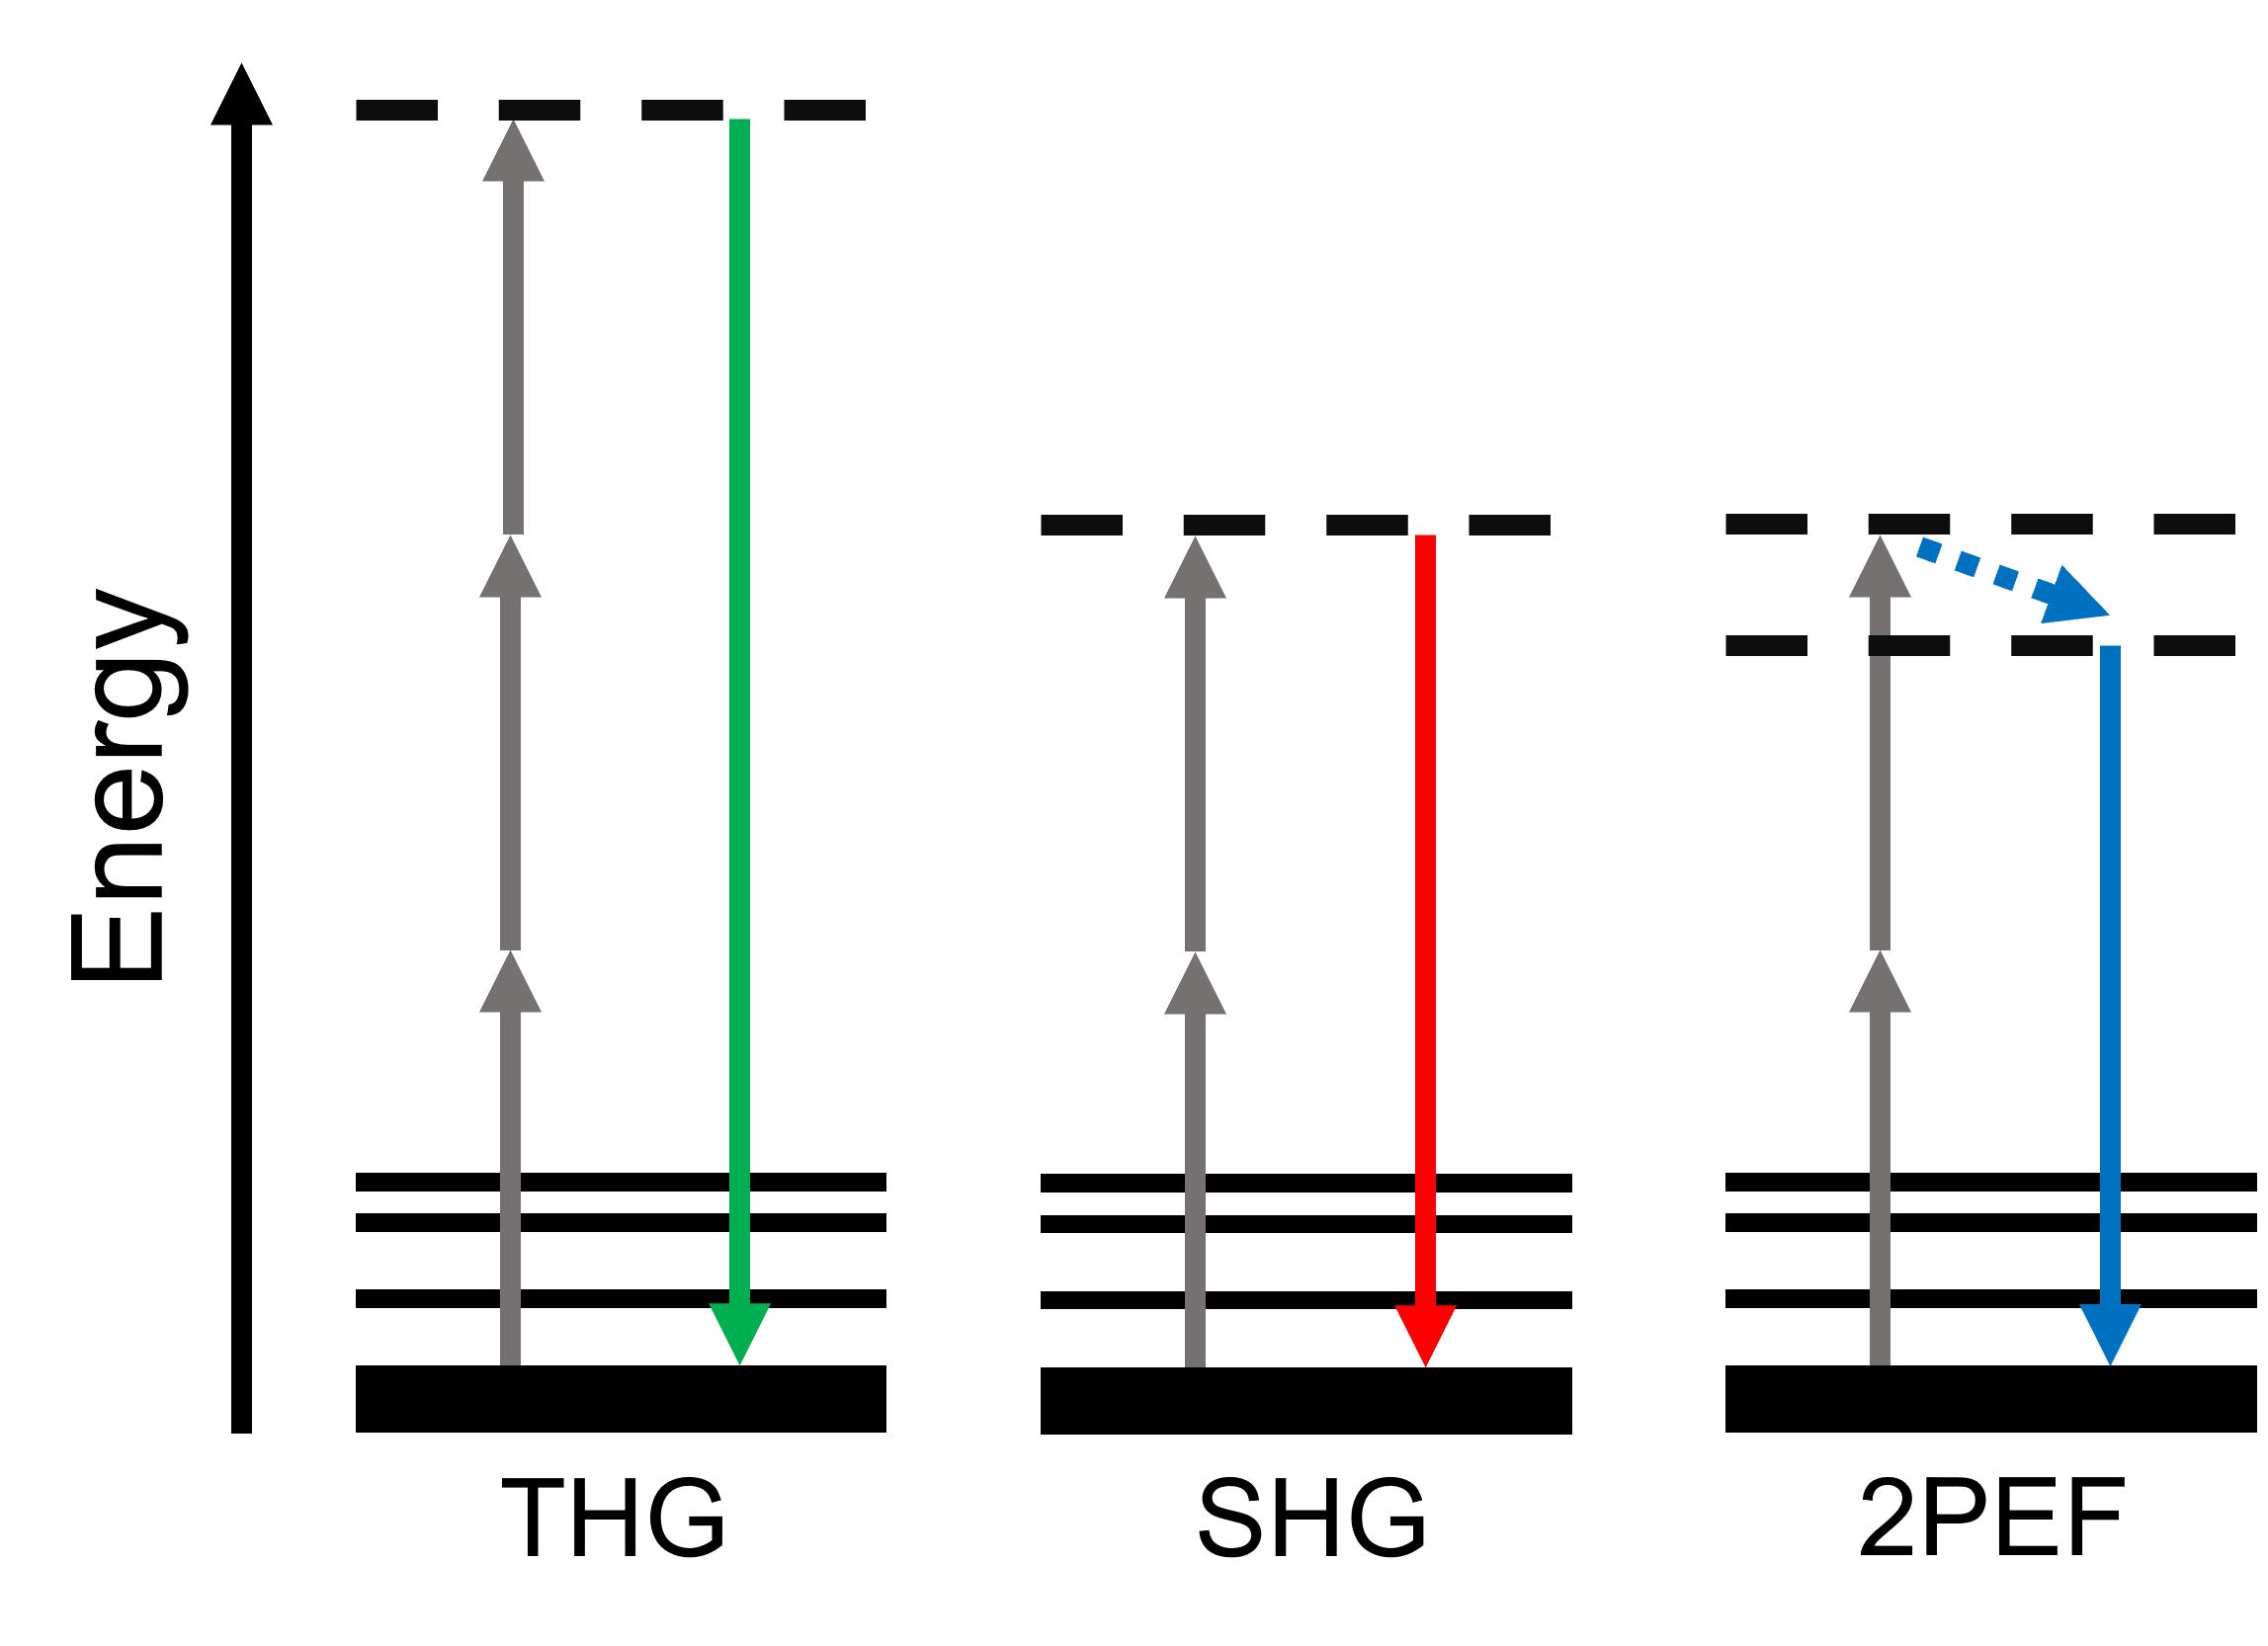
\includegraphics[width=\linewidth]{ANN/images/hhg-jablonski.png}
    \caption[HHG Jablonski diagram]{Jablonski diagram for third (THG) and second harmonic generation (SHG), and two-photon excitation fluorescence (2PEF).}
    \label{fig:hhg-jablonski}
\end{figure}
